\documentclass[12pt,oneside,english,a4paper]{article}
\usepackage{babel}
\usepackage[utf8]{inputenc}
\usepackage[T1]{fontenc}
\usepackage{color}
\usepackage{graphicx}
\usepackage{wallpaper}
\usepackage{wrapfig,booktabs}

\usepackage{fancyhdr}

\usepackage{fourier-orns}
\newcommand{\dash}{\noindent \newline\textcolor{black}{\hrulefill~ \raisebox{-2.5pt}[10pt][10pt]{\leafright \decofourleft \decothreeleft  \aldineright \decotwo \floweroneleft \decoone   \floweroneright \decotwo \aldineleft\decothreeright \decofourright \leafleft} ~  \hrulefill}}

\usepackage{titlesec}
\titleformat*{\section}{\it\huge\bfseries}
\titleformat*{\subsection}{\it\huge\bfseries}
\titleformat*{\subsubsection}{\it\LARGE\bfseries}
\titleformat*{\paragraph}{\huge\bfseries}
\titleformat*{\subparagraph}{\LARGE\bfseries}

\usepackage[left=20px,right=20px,top=50px,bottom=50px,paperwidth=8in,paperheight=12in]{geometry}

\usepackage[cjk]{kotex}
\usepackage{amsthm} 
\usepackage{amsmath} 
\usepackage{amsfonts}
\usepackage{enumerate} 
\usepackage{cite}
\usepackage{graphics} 
\usepackage{graphicx,lscape} 
\usepackage{subcaption}
\usepackage{algpseudocode}
\usepackage{algorithm}
\usepackage{titlesec}
\usepackage{cite, url}
\usepackage{amssymb}

\def\bk{\paragraph{\Large$$}\Large}
\def\ck{\paragraph{\Large$\bullet$}\Large}
\def\sol{\paragraph{\Large(sol)}\Large}
\def\pf{\paragraph{\Large(pf)}\Large}
\def\note{\paragraph{\Large\textit{\underline{note:}}}\Large}
\def\ex{\paragraph{\Large\textit{example:}}\Large}
\newcommand{\para}[1]{\paragraph{\Large\it\underline{\textbf{#1:}}}\Large}
\newcommand{\parablue}[1]{\paragraph{\Large\textcolor{blue}{\it\underline{\textbf{#1:}}}}\Large}
\newcommand{\parared}[1]{\paragraph{\Large\textcolor{red}{\it\underline{\textbf{#1:}}}}\Large}


\def\one{\paragraph{\Large(1)}\Large}
\def\two{\paragraph{\Large(2)}\Large}
\def\three{\paragraph{\Large(3)}\Large}
\def\four{\paragraph{\Large(4)}\Large}
\def\five{\paragraph{\Large(5)}\Large}
\def\six{\paragraph{\Large(6)}\Large}
\def\seven{\paragraph{\Large(7)}\Large}
\def\eight{\paragraph{\Large(8)}\Large}
\def\nine{\paragraph{\Large(9)}\Large}
\def\ten{\paragraph{\Large(10)}\Large}

\def\cka{\paragraph{\Large(a)}\Large}
\def\ckb{\paragraph{\Large(b)}\Large}
\def\ckc{\paragraph{\Large(c)}\Large}
\def\ckd{\paragraph{\Large(d)}\Large}
\def\cke{\paragraph{\Large(e)}\Large}
\def\ckf{\paragraph{\Large(f)}\Large}
\def\ckg{\paragraph{\Large(g)}\Large}
\def\ckh{\paragraph{\Large(h)}\Large}
\def\cki{\paragraph{\Large(i)}\Large}
\def\ckj{\paragraph{\Large(j)}\Large}

\newcommand{\bs}[1]{\mbox{\boldmath $#1$}}

\newcommand{\bsa}{\mbox{\boldmath $a$}}
\newcommand{\bsb}{\mbox{\boldmath $b$}}
\newcommand{\bsc}{\mbox{\boldmath $c$}}
\newcommand{\bsd}{\mbox{\boldmath $d$}}
\newcommand{\bse}{\mbox{\boldmath $e$}}
\newcommand{\bsf}{\mbox{\boldmath $f$}}
\newcommand{\bsg}{\mbox{\boldmath $g$}}
\newcommand{\bsh}{\mbox{\boldmath $h$}}
\newcommand{\bsi}{\mbox{\boldmath $i$}}
\newcommand{\bsj}{\mbox{\boldmath $j$}}
\newcommand{\bsk}{\mbox{\boldmath $k$}}
\newcommand{\bsl}{\mbox{\boldmath $l$}}
\newcommand{\bsm}{\mbox{\boldmath $m$}}
\newcommand{\bsn}{\mbox{\boldmath $n$}}
\newcommand{\bso}{\mbox{\boldmath $o$}}
\newcommand{\bsp}{\mbox{\boldmath $p$}}
\newcommand{\bsq}{\mbox{\boldmath $q$}}
\newcommand{\bsr}{\mbox{\boldmath $r$}}
\newcommand{\bss}{\mbox{\boldmath $s$}}
\newcommand{\bst}{\mbox{\boldmath $t$}}
\newcommand{\bsu}{\mbox{\boldmath $u$}}
\newcommand{\bsv}{\mbox{\boldmath $v$}}
\newcommand{\bsw}{\mbox{\boldmath $w$}}
\newcommand{\bsx}{\mbox{\boldmath $x$}}
\newcommand{\bsy}{\mbox{\boldmath $y$}}
\newcommand{\bsz}{\mbox{\boldmath $z$}}

\newcommand{\bfa}{\mbox{$\bf{a}$}}
\newcommand{\bfb}{\mbox{$\bf{b}$}}
\newcommand{\bfc}{\mbox{$\bf{c}$}}
\newcommand{\bfd}{\mbox{$\bf{d}$}}
\newcommand{\bfe}{\mbox{$\bf{e}$}}
\newcommand{\bff}{\mbox{$\bf{f}$}}
\newcommand{\bfg}{\mbox{$\bf{g}$}}
\newcommand{\bfh}{\mbox{$\bf{h}$}}
\newcommand{\bfi}{\mbox{$\bf{i}$}}
\newcommand{\bfj}{\mbox{$\bf{j}$}}
\newcommand{\bfk}{\mbox{$\bf{k}$}}
\newcommand{\bfl}{\mbox{$\bf{l}$}}
\newcommand{\bfm}{\mbox{$\bf{m}$}}
\newcommand{\bfn}{\mbox{$\bf{n}$}}
\newcommand{\bfo}{\mbox{$\bf{o}$}}
\newcommand{\bfp}{\mbox{$\bf{p}$}}
\newcommand{\bfq}{\mbox{$\bf{q}$}}
\newcommand{\bfr}{\mbox{$\bf{r}$}}
\newcommand{\bfs}{\mbox{$\bf{s}$}}
\newcommand{\bft}{\mbox{$\bf{t}$}}
\newcommand{\bfu}{\mbox{$\bf{u}$}}
\newcommand{\bfv}{\mbox{$\bf{v}$}}
\newcommand{\bfw}{\mbox{$\bf{w}$}}
\newcommand{\bfx}{\mbox{$\bf{x}$}}
\newcommand{\bfy}{\mbox{$\bf{y}$}}
\newcommand{\bfz}{\mbox{$\bf{z}$}}

\newcommand{\bsA}{\mbox{\boldmath $A$}}
\newcommand{\bsB}{\mbox{\boldmath $B$}}
\newcommand{\bsC}{\mbox{\boldmath $C$}}
\newcommand{\bsD}{\mbox{\boldmath $D$}}
\newcommand{\bsE}{\mbox{\boldmath $E$}}
\newcommand{\bsF}{\mbox{\boldmath $F$}}
\newcommand{\bsG}{\mbox{\boldmath $G$}}
\newcommand{\bsH}{\mbox{\boldmath $H$}}
\newcommand{\bsI}{\mbox{\boldmath $I$}}
\newcommand{\bsJ}{\mbox{\boldmath $J$}}
\newcommand{\bsK}{\mbox{\boldmath $K$}}
\newcommand{\bsL}{\mbox{\boldmath $L$}}
\newcommand{\bsM}{\mbox{\boldmath $M$}}
\newcommand{\bsN}{\mbox{\boldmath $N$}}
\newcommand{\bsO}{\mbox{\boldmath $O$}}
\newcommand{\bsP}{\mbox{\boldmath $P$}}
\newcommand{\bsQ}{\mbox{\boldmath $Q$}}
\newcommand{\bsR}{\mbox{\boldmath $R$}}
\newcommand{\bsS}{\mbox{\boldmath $S$}}
\newcommand{\bsT}{\mbox{\boldmath $T$}}
\newcommand{\bsU}{\mbox{\boldmath $U$}}
\newcommand{\bsV}{\mbox{\boldmath $V$}}
\newcommand{\bsW}{\mbox{\boldmath $W$}}
\newcommand{\bsX}{\mbox{\boldmath $X$}}
\newcommand{\bsY}{\mbox{\boldmath $Y$}}
\newcommand{\bsZ}{\mbox{\boldmath $Z$}}

\newcommand{\bfA}{\mbox{$\bf{A}$}}
\newcommand{\bfB}{\mbox{$\bf{B}$}}
\newcommand{\bfC}{\mbox{$\bf{C}$}}
\newcommand{\bfD}{\mbox{$\bf{D}$}}
\newcommand{\bfE}{\mbox{$\bf{E}$}}
\newcommand{\bfF}{\mbox{$\bf{F}$}}
\newcommand{\bfG}{\mbox{$\bf{G}$}}
\newcommand{\bfH}{\mbox{$\bf{H}$}}
\newcommand{\bfI}{\mbox{$\bf{I}$}}
\newcommand{\bfJ}{\mbox{$\bf{J}$}}
\newcommand{\bfK}{\mbox{$\bf{K}$}}
\newcommand{\bfL}{\mbox{$\bf{L}$}}
\newcommand{\bfM}{\mbox{$\bf{M}$}}
\newcommand{\bfN}{\mbox{$\bf{N}$}}
\newcommand{\bfO}{\mbox{$\bf{O}$}}
\newcommand{\bfP}{\mbox{$\bf{P}$}}
\newcommand{\bfQ}{\mbox{$\bf{Q}$}}
\newcommand{\bfR}{\mbox{$\bf{R}$}}
\newcommand{\bfS}{\mbox{$\bf{S}$}}
\newcommand{\bfT}{\mbox{$\bf{T}$}}
\newcommand{\bfU}{\mbox{$\bf{U}$}}
\newcommand{\bfV}{\mbox{$\bf{V}$}}
\newcommand{\bfW}{\mbox{$\bf{W}$}}
\newcommand{\bfX}{\mbox{$\bf{X}$}}
\newcommand{\bfY}{\mbox{$\bf{Y}$}}
\newcommand{\bfZ}{\mbox{$\bf{Z}$}}

\DeclareMathOperator*{\argmin}{argmin} 
\DeclareMathOperator*{\argmax}{argmax} 

\usepackage[svgnames]{xcolor}
\usepackage{listings}

\lstset{language=R,
    basicstyle=\Large\tt,
    stringstyle=\color{DarkGreen},
    otherkeywords={0,1,2,3,4,5,6,7,8,9},
    morekeywords={TRUE,FALSE},
    deletekeywords={data,frame,length,as,character},
    %keywordstyle=\color{blue},
    commentstyle=\color{DarkGreen},
}

\CJKscale{0.9}
\begin{document}
\section{Ergodic}
\parared{Theorem} Let ${\cal G}=(V,{\boldsymbol E},{\boldsymbol W})$ be a weighted graph with $|V|=n$ and $f$ be a graph signal defined on ${\cal G}$. Let ${\cal H}(f,{\cal G};\tau)$ denote the heavy snow transformation of $f$. Then there exists a unique stationary distribution ${\boldsymbol \pi}^{\star}$ such that 
$
{\boldsymbol\pi}^{0}\prod_{\tau=1}^{\infty}{\boldsymbol P}^{\tau}={\boldsymbol \pi}^{\star}, 
$
where ${\boldsymbol P}^{\tau}$ is a transition matrix with the $(i,j)$th element $P_{ij}^{\tau}=\mbox{Prob}\big(v_j=\tilde{v}^{\tau}|v_i=\tilde{v}^{\tau-1}\big)$ and ${\boldsymbol\pi}^{0}=(1/n,\dots,1/n)^\top$.

\proof The necessary conditions for the ergodictiy of ${\boldsymbol{P}^{\tau}}$ are (i) irreducible and (ii) aperiodic. For (i) irreducible, it is clear due to $\gamma<1$. To show (ii), suppose that 
$
\mbox{gcd}\{\tau>0: \mbox{Prob}(\tilde v^{\tau}=v | \tilde v^{0}=u)>0\} \geq 2, 
$
where $\mbox{gcd}$ denotes the greatest common divisor. For all $v_i \in V$ and $\ell >0$, $P_{ii}^{\ell}$ should be $0$, contrary to the assumption. 

\note $\bsP$가 $\tau$에 따라 변화해도 상관없는지? 

\parared{Theorem} ${\cal G}=(V,\bsE,\bsW)$가 $\max_{i,j}|f(v_i)-f(v_j)|<\infty$인 regular graph라면 모든 고정된 $i,j$에 대하여 아래가 성립한다. 
\[
p_{12}^{\tau} = \frac{W_{12}}{\sum_{j=1}^{n}W_{1j}}+o(1) \quad \mbox{ for all } i,j.
\]
여기에서 
\[
p_{12}^\tau:=Prob(T^{\tau}=2|T^{\tau-1}=1)=
\begin{cases}
\frac{d(v_2)}{\sum_{i=1}^{n}d(v_i)} & {\cal U}^{\tau-1}=\emptyset \\ 
\frac{1}{|{\cal U}^{\tau-1}|} & {\cal U}^{\tau-1} \neq \emptyset \mbox{ and } v_1 \in {\cal U}^{\tau-1}\\ 
0 & {\cal U}^{\tau-1} \neq \emptyset \mbox{ and } v_1 \notin {\cal U}^{\tau-1}
\end{cases}
\]
\proof 
아래와 같이 쓰자.
\begin{align*}
& p_{12}^{\tau}=a^{\tau}+b^{\tau}+0 \\ 
& a^{\tau} = I({\cal U}^{\tau-1}=\emptyset)\times \frac{d(v_2)}{\sum_{i=1}^n d(v_i)}=I({\cal U}^{\tau-1}=\emptyset)\frac{d(v_2)}{d} \\
& b^{\tau} = I({\cal U}^{\tau-1}\neq\emptyset)I(1\in{\cal U}^{\tau-1})\times \frac{1}{|{\cal U}^{\tau-1}|} 
\end{align*}
그런데 $\frac{I(v_1\in{\cal U}^{\tau-1})}{|{\cal U}^{\tau-1}|}=\frac{d(v_1)}{d}+o_p(1)$ 이므로 $b^{\tau}=I({\cal U}^{\tau-1}\neq \emptyset)\frac{d(v_1)}{d}+o_p(1)$ 이다. 정리하면
\begin{align*}
& a^{\tau} =I({\cal U}^{\tau-1}=\emptyset)\frac{d(v_2)}{d} \\
& b^{\tau} = I({\cal U}^{\tau-1}\neq\emptyset)\frac{d(v_1)}{d}+o_p(1)
\end{align*}
따라서 만약에 $d(v_1)=d(v_2)$라면 
\[
p_{12}^{\tau}=a^{\tau}+b^{\tau}=\frac{d(v_1)}{d}+o_p(1)=\frac{d(v_2)}{d}+o_p(1)
\]
그런데 $\frac{d(v_2)}{d}=\frac{W_{12}}{\sum_jW_{1j}}$이므로 증명끝. 

\section{예제2에 대한 백업 (1)}
\parared{Theorem}
\ck 빨주노초파남보의 7개의 노드가 있다고 하자. 즉 $V=\{1,2,3,\dots,7\}$이라고 하자. 그리고 이들이 서로 링형태로 연결되어 있다고 가정하자. 

\para{주장1}: $\ell$시점에서 그림1의 각 지형이 형성될 확률은 모두 같다. 

\begin{figure}[h]
\center
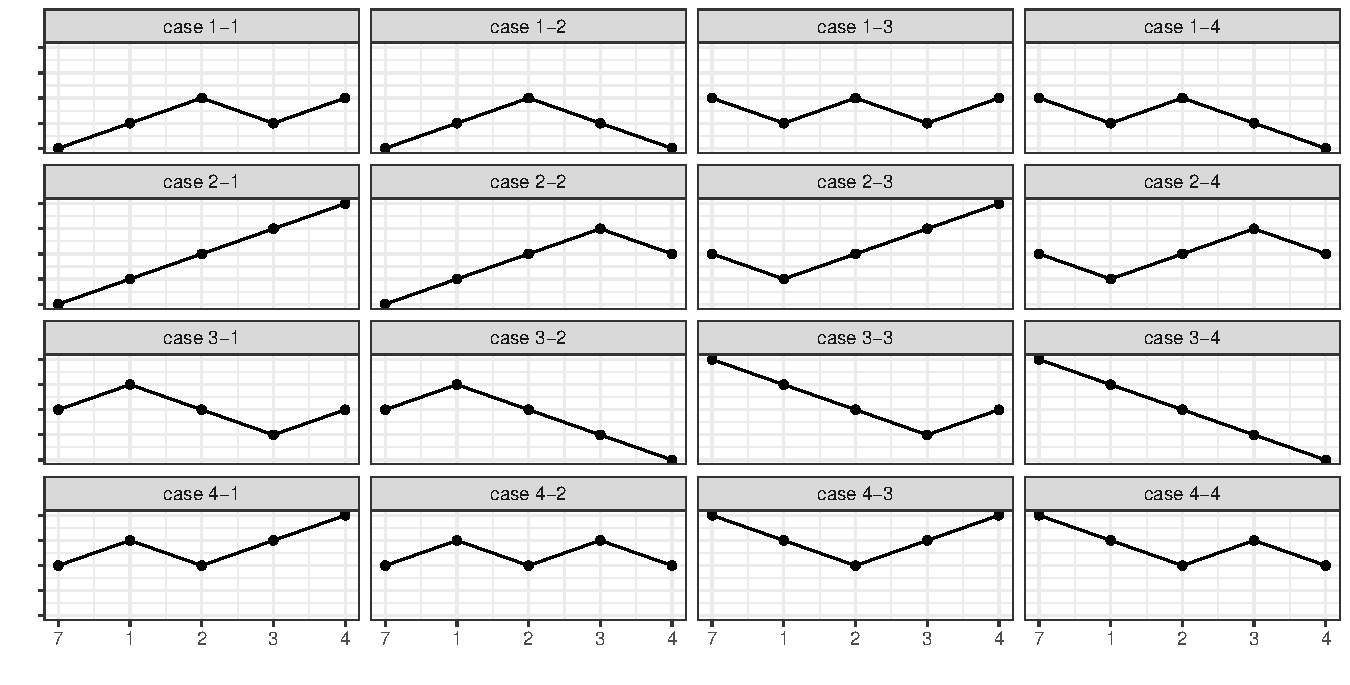
\includegraphics[width=1\textwidth]{Fig1.pdf}
\caption{가능한 지형들의 경우들}
\end{figure}
\dash

\para{주장2}: $\tau=\ell-1$에서 성립한다면 $\tau=\ell$에서도 성립한다. 

\para{주장2의 증명}
\ck 아래를 보이면 된다. 
\[
\Sigma_{13}^{\ell}-\Sigma_{12}^{\ell}=\Sigma_{13}^{\ell-1}-\Sigma_{12}^{\ell-1}+(h_{1}^{\ell}-h_3^{\ell})^2-(h_{1}^{\ell}-h_2^{\ell})^2\geq 0
\]
그런데 $\Sigma_{13}^{\ell-1}-\Sigma_{12}^{\ell-1}>0$ 이므로 아래를 보이면 충분하다. 
\begin{align*}
& A:=(h_{1}^{\ell}-h_3^{\ell})^2-(h_{1}^{\ell}-h_2^{\ell})^2 \\
& =(h_1^{\ell-1}+\xi_{1}^{\ell}-h_3^{\ell-1}-\xi_3^{\ell})^2-(h_1^{\ell-1}+\xi_{1}^{\ell}-h_2^{\ell-1}-\xi_2^{\ell})^2 \\ 
& =(h_1^{\ell-1}-h_3^{\ell-1})^2+(\xi_1^{\ell}-\xi_3^{\ell})^2-2(h_1^{\ell-1}-h_3^{\ell-1})(\xi_1^{\ell}-\xi_3^{\ell}) \\
&\quad - (h_1^{\ell-1}-h_2^{\ell-1})^2-(\xi_1^{\ell}-\xi_2^{\ell})^2+2(h_1^{\ell-1}-h_2^{\ell-1})(\xi_1^{\ell}-\xi_2^{\ell})\geq 0
\end{align*}
그런데 
\[
(h_1^{\ell-1}-h_3^{\ell-1})^2-(h_1^{\ell-1}-h_2^{\ell-1})^2 \geq 0 
\]
이므로 아래만 보이면 된다. 
\[
(\xi_1^{\ell}-\xi_3^{\ell})^2-2(h_1^{\ell-1}-h_3^{\ell-1})(\xi_1^{\ell}-\xi_3^{\ell})-(\xi_1^{\ell}-\xi_2^{\ell})^2+2(h_1^{\ell-1}-h_2^{\ell-1})(\xi_1^{\ell}-\xi_2^{\ell})\geq 0
\]
아래와 같이 나누자. 
\[
\textcolor{orange}{A_1:=(\xi_1^{\ell}-\xi_3^{\ell})^2-(\xi_1^{\ell}-\xi_2^{\ell})^2}
\]
\[
\textcolor{orange}{A_2:=-2(h_1^{\ell-1}-h_3^{\ell-1})(\xi_1^{\ell}-\xi_3^{\ell})+2(h_1^{\ell-1}-h_2^{\ell-1})(\xi_1^{\ell}-\xi_2^{\ell})}
\]

\ck 먼저 $\ell-1$시점에서 눈이 갇힌 (blocked) 경우를 고려하자. 눈이 갇히고 노드 1에 왔다면 $A_1=0$ 이다. 따라서
\[
A=A_2=2b\left(h_3^{\ell-1}-h_2^{\ell-1}\right)
\]
블락된 이후 노드2로 왔다면 $A_1=-b^2$ 이고 
\[
A=-b^2+A_2=-b^2+2b(h_1^{\ell-1}-h_2^{\ell-1})=2b\left(h_2^{\ell-1}-h_1^{\ell-1}-\frac{b}{2}\right)
\]
블락된 이후 노드3으로 왔다면 $A_1=b^2$이고 
\[
A=b^2+A_2=b^2+2b(h_1^{\ell-1}-h_3^{\ell-1})=2b\left(h_1^{\ell-1}-h_3^{\ell-1}+\frac{b}{2}\right)
\]
블락된 이후에 각 경우에 대하여 평균적으로 $A$는
\[
2b\left( h_3^{\ell-1}-h_2^{\ell-1}+h_2^{\ell-1}-h_1^{\ell-1}-\frac{b}{2}+h_1^{\ell-1}-h_3^{\ell-1}+\frac{b}{2}\right)=0
\]
이는 지형에 상관없이 성립한다. 따라서 블락된 경우는 따질 필요가 없다. 

\ck $\ell$ 시점에서 눈이 쌓이는 경우는 아래의 경우가 있다. 
\begin{itemize}
\item $(\xi_1^\ell,\xi_2^\ell,\xi_3^\ell)=(0,0,0) \Longrightarrow A=0:=a_0$
\item $(\xi_1^\ell,\xi_2^\ell,\xi_3^\ell)=(\tilde{b},0,0) \Longrightarrow A=2\tilde{b}(h_3^{\ell-1}-h_2^{\ell-1}):=a_1$ 
\item $(\xi_1^\ell,\xi_2^\ell,\xi_3^\ell)=(0,\tilde{b},0) \Longrightarrow A=2\tilde{b}\left(h_2^{\ell-1}-h_1^{\ell-1}-\frac{\tilde{b}}{2}\right):=a_2$
\item $(\xi_1^\ell,\xi_2^\ell,\xi_3^\ell)=(0,0,\tilde{b}) \Longrightarrow A=2\tilde{b}\left(h_1^{\ell-1}-h_3^{\ell-1}+\frac{\tilde{b}}{2}\right):=a_3$
\end{itemize}
\note $a_1+a_2+a_3=0$임에 유의할것. 

\ck case2-1 $\sim$ case 3-4의 경우는 아래가 성립함이 자명함. (추후에 좀더 엄밀하게 서술할것임) 
\[
\Sigma_{13}^{\ell}-\Sigma_{12}^{\ell}\geq0 
\]

\parared{case 1-1 $\sim$ 1-4} 
\ck cases 1-1의 경우 (7번노드) $A=0$ (1번노드 )
\one $A=0$
\two $A=\frac{a_1+a_3}{2}$
\three block 
\four $A=\frac{3a_3}{4}$
\ck 따라서 $\frac{5a_1+2a_3}{4}$

\parared{1-2} 
\seven $A=0$
\one $A=0$
\two $A=\frac{a_1+a_3}{2}$
\three $A=0$
\four $A=0$
\ck 따라서 $\frac{2a_1+2a_3}{4}$.

\parared{1-3} 
\seven $A=\frac{3a_1}{4}$
\one block
\two $A=\frac{a_1+a_3}{2}$
\three block
\four $A=\frac{3a_3}{4}$
\ck 따라서 $\frac{4a_1+4a_3}{4}$.

\parared{1-4} 
\seven $A=\frac{3a_1}{4}$
\one block
\two $A=\frac{a_1+a_3}{2}$
\three $A=0$
\four $A=0$
\ck 따라서 $\frac{5a_1+2a_3}{4}$.

\ck 경우1을 종합하면 $\frac{16a_1+10a_3}{4}$

\parared{4-1} 
\seven $A=0$
\one $A=\frac{a_2}{2}$
\two block
\three $A=a_2$
\four $A=\frac{3a_3}{4}$
\ck 따라서 $\frac{6a_2+3a_3}{4}$

\parared{4-2} 
\seven $A=0$
\one $\frac{a_2}{2}$
\two block
\three $\frac{a_2}{2}$
\four $A=0$
\ck 종합 $\frac{4a_2}{4}$

\parared{4-3} 
\seven $A=\frac{3a_1}{4}$
\one $A=a_2$
\two block
\three $A=a_2$
\four $A=\frac{3a_3}{4}$
\ck 종합 $\frac{3a_1+8a_2+3a_3}{4}$

\parared{4-4} 
\seven $A=\frac{3a_1}{4}$
\one $A=a_2$
\two block
\three $A=\frac{a_2}{2}$
\four $A=0$
\ck 종합 $\frac{6a_2+3a_3}{4}$

\ck 경우4를 종합하면 $\frac{3a_1+18a_2+9a_3}{4}=\frac{16a_2+6a_3}{4}$
\ck 경우1과 경우4를 종합하면 $\frac{16a_1+10a_3}{4}+\frac{16a_2+6a_3}{4}=\frac{16a_1+16a_2+16a_3}{4}=0$

\dash

\parared{Theorem}
\ck 예제2에서 링과 링이 아닌 그룹은 분리가능함.

\dash 

\parared{Theorem}
\ck 변형된 예제1의 caseA의 경우 2개 그룹은 서로 분리가능함. 

\dash

\parared{Theorem (틀린듯)} Let ${\cal G}=(V,{\boldsymbol E},{\boldsymbol W})$ be a weighted graph with $|V|=n$ and $f$ be the graph function defined on ${\cal G}$. Assume that ${\cal G}$ is a regular graph. Suppose that $f(v_1),\dots,f(v_n)$ is $i.i.d$ random sample. Let ${\cal G}^{\tau}=(V,{\boldsymbol E},{\boldsymbol W}^{\tau})$be the weighted graph induced by the heavy snow transformation of $f$ ${\cal H}(f,{\cal G}; \tau)$. Then we have ${\boldsymbol W}^{\tau} \overset{p}{\to} {\boldsymbol W}$ element-wisely as $\tau \to \infty$.

\proof Using the results in Appendix A.2, we obtain $W_{ij}^{\tau} \sim N(T_{ij}(F),V_{ij}(T,F)/n)$, where $T_{ij}(F):=\int W_{ij}^{\tau}dF^{\tau}$. Note that $T_{ij}(F^{\tau}) \to 1 $ as $\tau \to \infty$ for $i\neq j$ and $T_{ij}(F^{\tau})=0$ for $i=j$. Further, we get $V_{ij}(T,F^{\tau})/n \to 0$ as $\tau \to \infty$ for all $i,j$. Thus ${\boldsymbol W}^{\tau} \overset{p}{\to} {\boldsymbol W}$ element-wisely as $\tau \to \infty$.

\parablue{Appendix 2}:
Let ${\cal G}=(V,{\boldsymbol E},{\boldsymbol W})$ be a weighted graph with $|V|=n$ and $f$ be a graph signal defined on ${\cal G}$. Assume that ${\cal G}$ is a regular graph. Suppose that $f(v_1),\dots,f(v_n)$ is $i.i.d$ random sample. Let ${\cal H}(f,{\cal G}; \tau)$ be the heavy snow transformation of $f$. \textcolor{red}{Since $f(v_i)$ is $i.i.d.$ random variable, ${\boldsymbol h}_i$ is $i.i.d.$ random vector with 
$
{\boldsymbol h}_1^{\tau},\dots,{\boldsymbol h}_n^{\tau} \sim F^{\tau}.
$}
Define a functional $T(F^{\tau})$ as 
$
T(F^{\tau}):=\int g({\boldsymbol h}) dF^{\tau}.
$
Let $F_n^{\tau}$ be an empirical distribution function of ${\boldsymbol h}_1^{\tau},\dots,{\boldsymbol h}_n^{\tau}$ defined as  
\[
F_n^{\tau}(m) :=\frac{1}{n}\sum_{i=1}^{n}1({\boldsymbol h}^{\tau}_i\leq t).
\]
From Glivenko-Cantelli Lemma,  we obtain $F_n^{\tau} \to F^{\tau}$. Thus, for a sufficiently large $n$, we can say that $F_n^{\tau}$ is a neighborhood of $F^{\tau}$. Hence, we have 
\begin{align*}
T(F_n^{\tau}) & \approx  T(F^{\tau})+\int IF(\boldsymbol{h}^{\tau},T,F^{\tau})d(F_n^{\tau}-F^{\tau}) \\
& = T(F^{\tau})+\int IF(\boldsymbol{h}^{\tau},T,F^{\tau}) dF_n^{\tau}, 
\end{align*}
where $IF({\boldsymbol h}^{\tau}; T,F^{\tau})= \lim_{t\downarrow 0}\frac{T((1-t)F^{\tau} + t \delta(\boldsymbol{h}) )-T(F^{\tau})}{t}$ is an influence function of $T$. Here, $\int IF(\boldsymbol{h}^{\tau},T,F^{\tau})dF^{\tau}=0$ is used. Therefore, it follows that  
\[
\sqrt{n}\Big(T(F_n^{\tau})-T(F^{\tau}) \Big) \to N(0,V(T,F^{\tau})), 
\]
where $V(T,F^{\tau})=\int IF(\boldsymbol{h}^{\tau},T,F^{\tau})^2 dF^{\tau}$. 

\parared{Theorem} 고정된 $n$에 대하여 
\begin{enumerate}[(i)]
\item $\theta_n^{\tau} \to \infty\quad as\quad \tau \to \infty$
\item $\max_{i,j}|f(v_i)-f(v_j)|=O(1)$
\end{enumerate}
이라면 아래를 만족하는 $\pi^{\star}$가 항상 존재한다. 
\[
\|\bs{\pi}-\bs{\pi}^{\star}\|_2^2=o(1)
\]
단 $\pi_i^{\tau}:=\frac{d_i^{\tau}}{\sum_{i}^nd_i^{\tau}}$, $d_i^{\tau}=\sum_{j=1}^{n}W_{ij}^{\tau}$ and $W_{ij}^{\tau}=\begin{cases}\exp\big(-\frac{1}{2}\frac{\Sigma_{ij}^{\tau}}{(\theta_n^{\tau})^2}\big) & i\neq j \\ 0 & i=j \end{cases}$

\proof 
모든 $v_i\in V$에 대하여 아래를 보이면 된다. 
\[
\pi_i^{\tau}-\pi_i^{\tau-1}=\frac{d_i^{\tau}}{d_1^{\tau}+\dots+d_n^{\tau}}-\frac{d_i^{\tau-1}}{d_1^{\tau-1}+\dots+d_n^{\tau-1}}=o(1)
\]
따라서 아래를 보이면 된다. 
\[
\frac{d_i^{\tau}}{d_1^{\tau}+\dots+d_n^{\tau}}=\frac{d_i^{\tau-1}}{d_1^{\tau-1}+\dots+d_n^{\tau-1}}+o(1)
\]

\parablue{case1} : $d_1^{\tau}+\dots+d_n^{\tau}=d_1^{\tau-1}+\dots+d_n^{\tau-1}$이라고 하자. 
\ck 아래를 보이기만 하면 된다. 
\[
d_i^{\tau}-d_i^{\tau-1}=o(1)
\]
그런데 
\[
d_i^{\tau}=W_{i1}^{\tau}+W_{i2}^{\tau}+\dots+W_{in}^{\tau}=W_{i2}^{\tau}+\dots+W_{in}^{\tau}
\]
이므로 아래를 보이면 된다. 
\[
(W_{i1}^{\tau}-W_{i1}^{\tau-1})+\dots+(W_{in}^{\tau}-W_{in}^{\tau-1})=o(1)
\]
결국 모든 $j$에 대하여 아래를 보이면 된다. 
\[
W_{ij}^{\tau}-W_{ij}^{\tau-1}=o(1)
\]
따라서 아래를 보이면된다. 
\[
\frac{W_{ij}^{\tau}}{W_{ij}^{\tau-1}}-1=o(1)
\]

\note 
아래를 관찰하자. 
\begin{align*}
W_{ij}^{\tau}&=e^{-\frac{\Sigma_{ij}^{\tau}}{2(\theta_n^{\tau})^2}}
=e^{-\frac{1}{2}\big(\frac{h_i^0-h_j^0}{\theta_n^{\tau}}\big)^2}
e^{-\frac{1}{2}\big(\frac{h_i^1-h_j^1}{\theta_n^{\tau}}\big)^2}
\dots
e^{-\frac{1}{2}\big(\frac{h_i^{\tau-1}-h_j^{\tau-1}}{\theta_n^{\tau}}\big)^2}
e^{-\frac{1}{2}\big(\frac{h_i^\tau-h_j^\tau}{\theta_n^{\tau}}\big)^2} \\
W_{ij}^{\tau-1}&=e^{-\frac{\Sigma_{ij}^{\tau-1}}{2(\theta_n^{\tau-1})^2}}
=e^{-\frac{1}{2}\big(\frac{h_i^0-h_j^0}{\theta_n^{\tau-1}}\big)^2}
e^{-\frac{1}{2}\big(\frac{h_i^1-h_j^1}{\theta_n^{\tau-1}}\big)^2}
\dots
e^{-\frac{1}{2}\big(\frac{h_i^{\tau-1}-h_j^{\tau-1}}{\theta_n^{\tau-1}}\big)^2}
\end{align*}

\ck 따라서 
\[
\frac{W_{ij}^{\tau}}{W_{ij}^{\tau-1}}
=A_1 \times \dots \times A_{\tau-1}\times A_\tau
\]
이때 
\begin{align*}
A_0&=\exp\left(-\frac{1}{2}\left(\frac{1}{(\theta_n^\tau)^2}-\frac{1}{(\theta_n^{\tau-1})^2}\right)(h_i^0-h_j^0)^2\right) \\
A_1&=\exp\left(-\frac{1}{2}\left(\frac{1}{(\theta_n^\tau)^2}-\frac{1}{(\theta_n^{\tau-1})^2}\right)(h_i^1-h_j^1)^2\right) \\
\dots \\
A_{\tau-1}&=\exp\left(-\frac{1}{2}\left(\frac{1}{(\theta_n^\tau)^2}-\frac{1}{(\theta_n^{\tau-1})^2}\right)(h_i^{\tau-1}-h_j^{\tau-1})^2\right) \\ 
A_{\tau}&=\exp\left(-\frac{1}{2}\frac{1}{(\theta_n^\tau)^2}(h_i^{\tau}-h_j^{\tau})^2\right)
\end{align*}

\one 그런데 
\[
\frac{1}{(\theta_n^\tau)^2}-\frac{1}{(\theta_n^{\tau-1})^2}=o(1)
\]
이다. 왜냐하면 $\left\{\frac{1}{(\theta_n^{\tau})^2}\right\}_{\tau=1}^{\infty}$이 수렴하는 수열이기 때문이다. (수렴하는 수열은 코시수열임) 
\two 또한 모든 $\tau$에 대하여 
\[
\max_{i,j}|h_i^{\tau}-h_j^{\tau}|=O(1)
\]
이다. (한쪽에만 눈이 쌓일수는 없음.) 
\three $\exp$가 연속함수이므로 $A_1,\dots,A_{\tau-1}$는 모두 $1$로 수렴한다. 그리고 $A_{\tau}$ 역시 $1$로 수렴한다.

\ck 따라서 
\[
\frac{W_{ij}^{\tau}}{W_{ij}^{\tau-1}}
=1+o(1)
\]

\parablue{case2} :  이제 $d_1^{\tau}+\dots+d_n^{\tau}\neq d_1^{\tau-1}+\dots+d_n^{\tau-1}$ 라고 하자. 아래를 정의하자. 
\begin{align*}
&d^{\tau-1}=d_1^{\tau-1}+\dots+d_n^{\tau-1} \\
&d^{\tau}=d_1^{\tau}+\dots+d_n^{\tau} \\
& \tilde{d}^{\tau}=\max(d^{\tau},d^{\tau-1})
\end{align*}
Clearly,
\[
\tilde{d}^{\tau}=O(1)
\]
따라서 case1 을 반복하면 증명이 된다. 

\parared{lem} (1) $\cal G=(V,\bsE,\bsW)$를 모든 엣지가 연결된 레귤러 그래프라고 하자. 즉 $\bsW=\bsJ-\bsI$. (2) $f_1,\dots f_{100} \overset{iid}{\sim} N(\mu_1,1)$. 그러면 아래가 성립한다. 
\[
\bsW^{\tau} \overset{p}{\to} \bsJ-\bsI
\]

\parared{lem} (1) $\cal G=(V,\bsE,\bsW)$를 모든 엣지가 연결된 레귤러 그래프라고 하자. 즉 $\bsW=\bsJ-\bsI$. (2) $f_1,\dots f_{50} \overset{iid}{\sim} N(\mu_1,1)$ and $f_{51},\dots,f_{100} \overset{iid}{\sim} N(\mu_2,1)$. 그러면 아래가 성립한다. 
\[
\bsW^{\tau} \overset{p}{\to} \begin{bmatrix}\bsJ-\bsI & \bf{0} \\ \bf{0} & \bsJ-\bsI \end{bmatrix}
\]

\dash 
\parared{thm} 눈을 쌓을수록 노드정보를 상실한다. HST는 노드정보와 그래프도메인에서의 정보를 연속적으로 변화시키는 장치이다. 
\note 단순히 노드에서의 거리와 그래프도메인의 거리를 가중평균한것과 무슨 차이일까? 


\end{document}

